\chapter{Background}
%The background should set the project into context by motivating the subject matter and relating it to existing published work. The background will include a critical evaluation of the existing literature in the area in which your project work is based and should lead the reader to understand how your work is motivated by and related to existing work.

For my BSc individual project, I will be researching procedural content generation (PCG) algorithms and then implementing them each in a small 3D game made with the Godot Engine (and its domain-specific GDScript language).

\section{Procedural Generation: Background}

\href{https://en.wikipedia.org/wiki/Procedural_generation}{Procedural content generation} (usually referred to as simply ``procedural generation") refers to the creation of levels and other game objects programmatically and algorithmically, in lieu of a human being doing all the work. While procedural generation algorithms can be used to generate a myriad of things, from textures (for things like trees and clouds) to music (``generative music," as coined by legendary musician Brian Eno), by far its most common context is in automated level design, generating level layouts algorithmically in lieu of work from level designers. Game developers may opt to use procedural generation to save time and money designing levels or show off technical prowess in their games.

\href{https://en.wikipedia.org/wiki/Procedural\_generation#Video\_games}{Procedural generation in video games has a rich history.} Pioneering games such as Rogue (1980) took direct influence from tabletop role-playing games such as Dungeons and Dragons, and thus had a player navigate a randomly-generated world that expanded further as they went on. Such games spawned the \emph{roguelike} and \emph{roguelite} genres, which experienced immense popularity in the last decade. In the realm of first-person shooters, 2004's .kkrieger, as seen in Figure \ref{fig:kkrieger}, used procedural generation to create intricate 3D levels and fit them all into a game that takes up just 96 kilobytes of space. 

\begin{figure}[H]
	\centering
	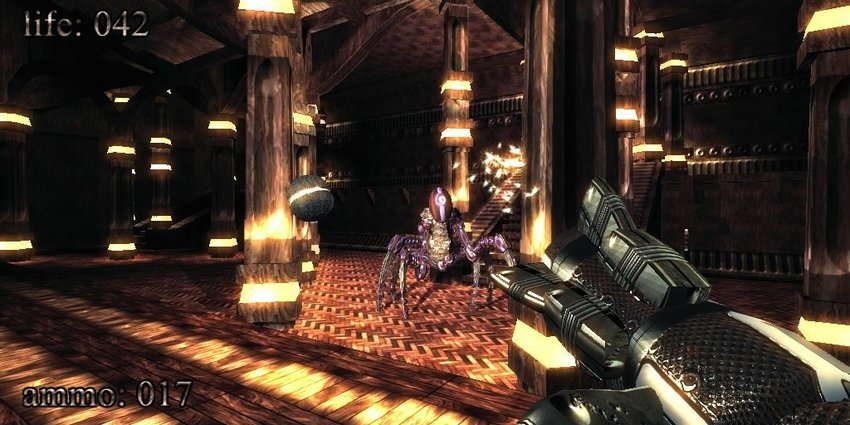
\includegraphics[width=0.75\textwidth]{Images/kkrieger.png}
	\caption{The game .kkrieger, which uses procedural generation to design maps while keeping the game at a 96 kilobyte file size.\cite{pcgvirtualworld}}
	\label{fig:kkrieger}
\end{figure}

Other games that use procedural generation in its levels include Elite (originally published in 1984), Elite: Dangerous (2012), Minecraft (2009), No Man's Sky (2012) and Spelunky (2013). \href{https://youtu.be/Uqk5Zf0tw3o}{The latter game's use of procedural generation has notably been covered by video games journalist Mark Brown in a YouTube video.}

\begin{figure}[H]
	\centering
	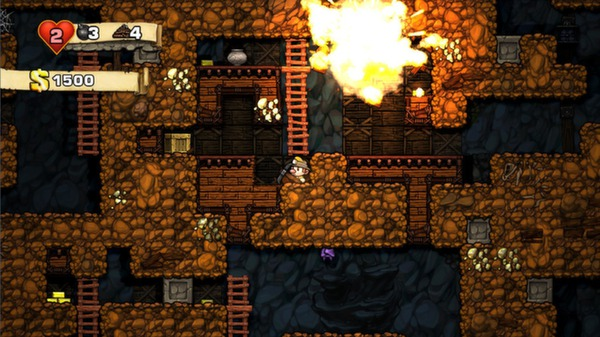
\includegraphics[width=0.7\textwidth]{Images/spelunky.jpg}
	\caption{\href{https://spelunkyworld.com/}{The roguelike game Spelunky}, which uses procedural generation to build intricate levels for the player character to explore.\\Source: \link{https://store.steampowered.com/app/239350/Spelunky/}}
	\label{fig:spelunky}
\end{figure}

In many cases, these games end up having a \textbf{large} number of different environments that each game could generate for its players. However, by procedurally generating them upon the \textit{loading} of the game level, in lieu of loading a layout from disk, they can save a lot of space (albeit with a considerable need for processing power, depending on the game's and algorithms' performance), as seen in Figure \ref{fig:kkrieger}.

Using one or some different procedural generation algorithms, such as the use of Perlin, Simplex or other noise, Voronoï disks and also poisson disk generation, among others, games can load a seed to randomly generate a level every time it is played, meaning no two playthroughs of a game with procedurally generated content are ever the same.

\section{Justifying My Choice of Engine: Godot}

While a myriad of resources exist for procedurally generated game contents exist for Unity and Unreal, I want to implement them in Godot, for several reasons:

\begin{itemize}
	\item It's the engine I have the most experience with, having already developed 2 published web games with it.
	\item It's not got as many resources on procedural generation compared to Unity, Unreal and some other popular game engines, particularly on the side of academic research (that is, there aren't as many papers on procedural generation that pertain to Godot as they do to Unity, Unreal and other engines).
	\begin{itemize}
		\item However, it is still very powerful and feature-rich (it has its own Open Simplex noise class, for example) and I'm sure I can make procedural generation algorithms work on it.
	\end{itemize}
	\item Compared to Unity and Unreal, Godot is a very light engine with a feature-rich editor, clocking in at under 100MB, with editors for Windows, macOS, Linux and even the web browser. 
\end{itemize}

By the end of my allotted time, I plan to have implemented several procedurally generated environments in small Godot games, using a myriad of methods (such as Voronoï cells and poisson disk generation) in a myriad of contexts (anything from platformers to first-person games). With these games, I plan for the final report to be the centrepiece of my project, with it containing my research on how each environment was implemented, as well as my findings on the algorithms themselves and how they work.

This is somewhere between a research-oriented project and an implementation-oriented project, as while the produced software artifacts provide valid proof of my understanding of some commonly used procedural generation algorithms and how to implement them in Godot, it is also about how I understand their workings. Nonetheless, the implementations provide the weight behind my project's motivations and are the main focus of this dissertation. They will prove that Godot is just as adept at procedural content generation as the other major players in the game engine space, and I will have gained a wealth of knowledge on PCG in the process.

\subsection{Note on Differing Versions of Godot}

Godot currently is at version 4, which finally received a stable release in 4\textsuperscript{th} March after years of development, but concurrently there is also Godot 3, the previous stable version which is now a \textbf{L}ong-\textbf{T}erm \textbf{S}upport release. The latter version of Godot contains several new features and breaking changes, so any project made in Godot 3 won't readily be compatible with Godot 4 (and vice-versa) without making the necessary changes and conversions. I have access to both versions of Godot and, for all the Godot projects I made and used in this project, I have used Godot 4. Any references to other Godot 3 projects will be clearly denoted as such.

\section{Justifying My Choice of Scenario: A 2D tile-map RPG-style roaming game}

The scenario of my choosing involves a monochrome tile-map created by Kenney.nl in a 2D RPG setting, in which the player character is a hollow ``Golem" that is trying to search for and obtain a ring among a large 72x40 village, filled with trees, buildings and emptiness. The player can ``chow down" trees by simply going to the cells where trees are and making them disappear. However, the player \textit{will} stop at and collide with any buildings in the tile map. When the player collects the ring, they win the game and are able to either close the window or generate a new village to try and collect \textit{another} ring.

The size of the tile map is determined by taking the window size, 1152x640 in \textbf{all} implementations, and then dividing it with the cell size, 16x16 in \textbf{all} implementations (again), hence returning a 72x40 tile map size. Using a large tile map like this, with 2880 available cells in total, allows for easy stress-testing of the algorithms, making them generate level layouts that are sufficiently large enough to produce a quantifiable performance result and time that can be easily compared across implementations, such that we can easily measure how one performs over the other. The use of a tile map \textit{this} large with PCG algorithms also makes sense from a game developer's perspective as designing level layouts this large by hand, with such a small cell size as well (inherited from the size of the tile map assets), would add additional time and labour costs to them. 

The use of a tiled role-playing game scenario, adapted to already-existing procedural generation algorithms, is relatively unusual in the context of procedural generation. However, it \textit{will} allow me to go a degree beyond the scope of what is usually done for procedural content generation in games, which is usually seen in 2D and 3D roguelikes and platformers, as well as some other world-building games such as Minecraft and Terrraria. The ability for the player character to consume trees and remove them from the level layout by moving into them allows that player to easily move around in what would otherwise be very crowded level layouts that would have been near-impossible to traverse. The addition of said player character, as well as the end goal of obtaining a randomly-placed ring within the given level, adds weight to the algorithms' practical use in games made with Godot, and not just for show or solely as demonstrations. 

\section{Justifying My Choice of Algorithms for the Above Scenario}

For this project, I intend to use the following procedural content generation algorithms within my scenario:

\begin{enumerate}
    \item Lindenmayer Systems (or L-Systems)
    \item Perlin and Simplex Noise
    \item Poisson Disk Sampling/Distribution
    \item Voronoï Cells/Diagrams
\end{enumerate}

Using an L-System for generating a level layout is relatively uncommon, compared to its use in generating structures such as trees and buildings. However, I plan to integrate a deterministic context-free L-System (or a ``D0L-System") into an implementation of my scenario so I can compare it performance-wise to the other algorithms, and see how the repeated patterns generated from L-System grammars affect comparisons to the other implementations' level layouts. 

Perlin and Simplex Noise are far more commonly used for level layouts, so I created an implementation of my scenario with one to see how it compares with the others, speed-wise and layout-wise, and see if it really is the best for my chosen scenario.

Poisson Disk Sampling is usually used for item placement in planes, even with grids, so using a grid-like implementation, I will compare how it works with in a tile map and what differences arise between its use there and in its usual uses.

Though efforts were made to make level layouts as similar as possible across implementations, there are noticeable differences between the level layouts generated by L-Systems, Simplex noise and Poisson disk samples, and I touch on those when discussing those implementations in the relevant sections of my report.

In my research and implementation of Voronoï Cells I realised the level layouts it generated for my scenario were wholly unique, when compared with the other algorithm implementations, so much so that I had to re-shape my scenario and game mechanics to make both the scenario and levels generated fit with each other. Nonetheless, I believe this will serve as a unique comparison to the other algorithms and will serve as additional knowledge of procedural generation algorithms as well as more work towards understanding how to make them work in Godot games (as proven by my implementations).